\chapter{\textbf{Propiedades, modelos electromagnéticos del cuerpo humano y bandas de frecuencia}}\label{ch:cap3}

En este capítulo veremos una introducción a las propiedades electromagnéticas del cuerpo humano y las distintas bandas de frecuencia para Dispositivos Médicos Implantables. En la sección~\ref{sec:propiedades}, estudiaremos las propiedades y distintos modelos electromagnéticos del cuerpo humano. El análisis de las dos bandas principales de radiofrecuencia para los sistemas de comunicaciones de los DMI lo podemos ver en la sección~\ref{bandas}.


\section{Propiedades electromagnéticas y modelado del cuerpo humano}\label{sec:propiedades}

Antes de empezar a diseñar una antena microstrip, es importante conocer en qué entorno vamos a trabajar, es decir, sobre qué vamos a aplicar lo visto en el capítulo~\ref{ch:contexto}. En el presente estudio, dicho entorno es el \textbf{cuerpo humano}, el cual actúa de forma muy diferente con las diversas ondas electromagnéticas existentes. El cuerpo o tejidos humanos poseen propiedades electromagnéticas que pueden variar de forma sustancial, debido a que las ondas pueden variar tanto en amplitud, como en frecuencia, como en el modo en el que inciden en los tejidos. Es por esto, que los DMI junto a su sistema de comunicaciones, donde encontramos la antena microstrip, deben ser diseñados a la par que se dan las características del entorno de trabajo. Estas características de los tejidos son las que vamos a mencionar a continuación.

\subsection{Características de los tejidos humanos y/o animales}\label{subsec:caracteristicas-de-los-tejidos-humanos-y/o-animales}

Muchos autores han realizado estudios sobre las propiedades dieléctricas de los diferentes tejidos corporales, tanto humanos como animales, hasta la fecha. Existen datos tabulados~\cite{durney,geddes,stuchly} que van desde un rango de frecuencias desde 10 Hz hasta 30 GHz. Lo más difícil de estos estudios es siempre la tarea de conseguir tejidos o cuerpos vivos. La mayor parte de los recursos que se utilizan son organismos sin vida o tejidos muertos. En el caso de humanos, el estudio se centra en cadáveres a los que se les ha practicado la autopsia y en el caso de animales, son aquellos que se han sacados de mataderos: ovejas, cerdos, pollos, etc.

Para caracterizar un tejido animal o humano de manera electromagnética, tenemos tres importantes parámetros: la \textbf{permitividad relativa}, la \textbf{conductividad} y la \textbf{profundidad de penetración}.

\begin{itemize}
    \item La \textit{permitividad relativa} ($\epsilon_{r}$) hace referencia a cómo un campo eléctrico afecta a un medio y su tendencia a polarizarse: este parámetro es adimensional ya que se compara con la permitividad en el vacío ($\epsilon_{0}$). Se relaciona con el campo eléctrico y la densidad de flujo eléctrico de la siguiente manera:
    \begin{center}
        $D =  \epsilon E = \epsilon_{r}\epsilon_{0} E$
    \end{center}

    \item La \textit{conductividad} ($\sigma$) es la capacidad de un cuerpo para conducir corriente eléctrica, dejar paso a partículas cargadas: se mide en siemens por metro (S/m). El campo eléctrico es directamente proporcional a la distribución de corriente eléctrica gracias a esta magnitud:
    \begin{center}
        $J = \sigma E$
    \end{center}

    \item La \textit{profundidad de penetración} se definde como la longitud a la que las radiaciones electromagnéticas pueden llegar dentro de un material. Se mide simplemente en metros o milímetros y depende de los dos parámetros arriba mencionados, además de muchos otros, como la geometría del cuerpo, intensidad de la radiación, frecuencia, etc.
\end{itemize}

Podemos ver en la siguiente \textit{tabla \ref{tabla3.1}} extraída de \cite{yangtabla} algunos ejemplos de propiedades electromagnéticas de tejidos del cuerpo humano a una frecuencia de 2.45 GHz.

\begin{table}[h]
    \centering\scalebox{0.9}{
        \begin{tabular}{| c | c | c | c | c | c |}
            \hline
            \textbf{Nombre}       & \textbf{Conductividad} & \textbf{Permitividad} & \textbf{Profunidad}         \\
            \textbf{del tejido}   & \textbf{[S/m]}         & \textbf{relativa}     & \textbf{de penetración [m]} \\
            \hline
            \hline
            Cerebro, materia gris & 1.843                  & 48.83                 & 0.02031                     \\
            \hline
            Grasa                 & 0.10672                & 5.2749                & 0.11455                     \\
            \hline
            Músculo               & 1.773                  & 52.668                & 0.021886                    \\
            \hline
            Piel seca             & 1.4876                 & 37.952                & 0.022198                    \\
            \hline
            Piel húmeda           & 23.984                 & 20.369                & 0.0010736                   \\
            \hline
            Sangre                & 2.5878                 & 58.181                & 0.015842                    \\
            \hline
            \hline
        \end{tabular}}
    \caption{Propiedades electromagnéticas de tejidos humanos a 2.45 GHz.}
    \label{tabla3.1}
\end{table}

En la \textit{fig. \ref{fig:fig3.1}}, podemos ver la variación de los tres parámetros en músculo y grasa para un rango extenso de frecuencias.

\begin{figure}[!htb]
    \centering
    \subfigure[]{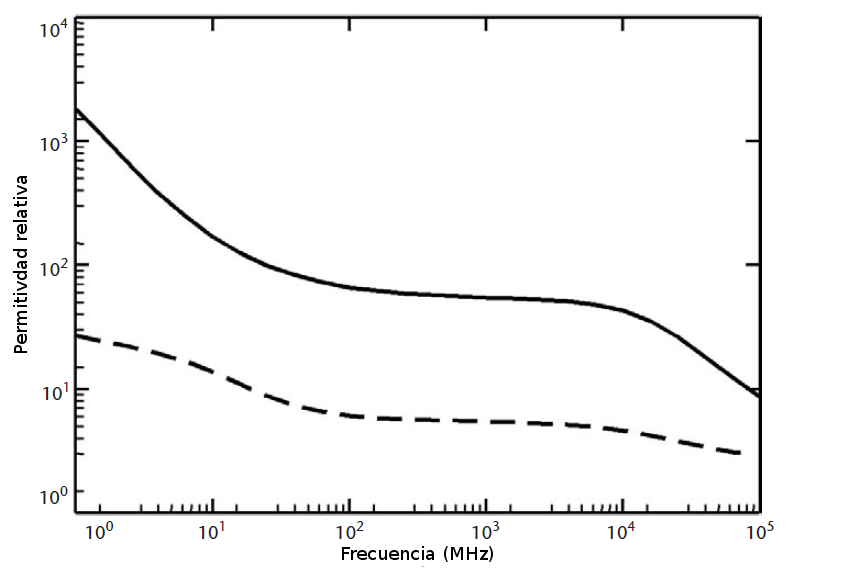
\includegraphics[scale=0.27]{./ContextoTecnologico/permitividad_relativa}}
    \subfigure[]{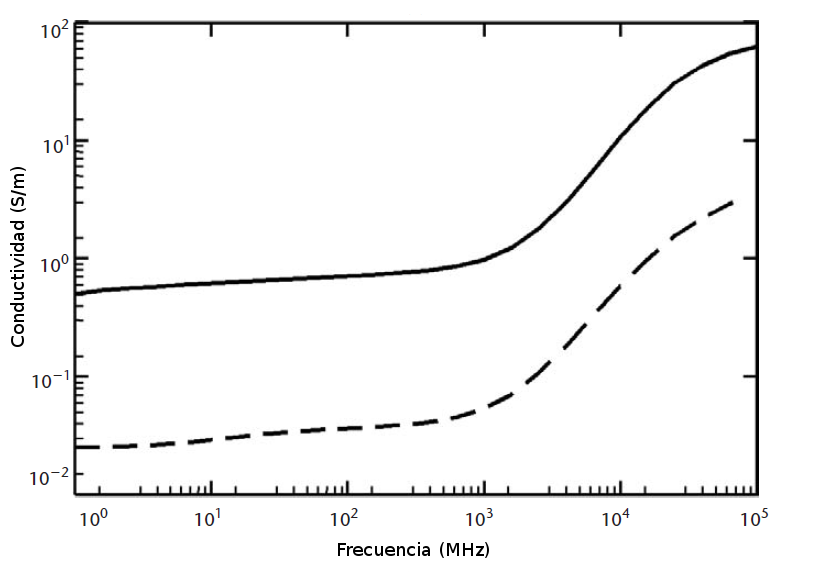
\includegraphics[scale=0.27]{./ContextoTecnologico/conductividad}}
    \subfigure[]{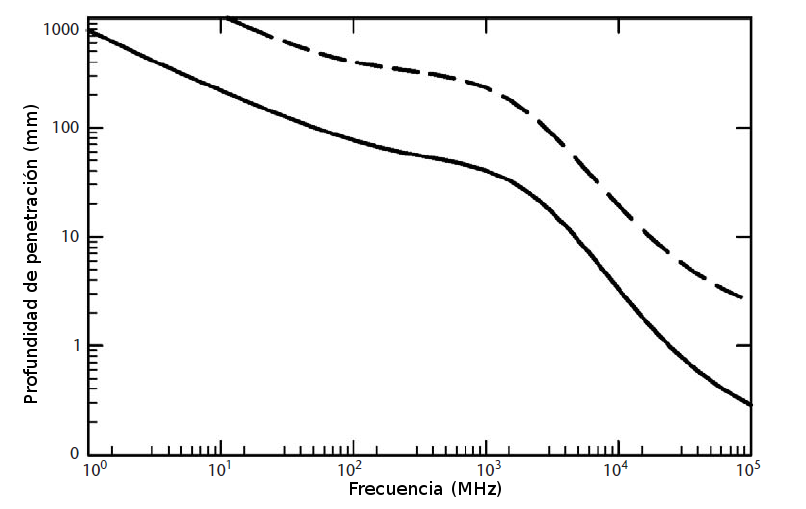
\includegraphics[scale=0.28]{./ContextoTecnologico/grado_de_penetracion}}
    \caption{Gráficas que representan distintas características de tejidos. En línea continua se representa el músculo y en discontinua grasa \cite{yang2}. En (a) permitividad relativa, en (b) conductividad y en (c) profundidad de penetración.}
    \label{fig:fig3.1}
\end{figure}

Las gráficas nos muestran una serie de características a destacar. Quedan recogidas en los siguientes puntos \cite{gabriel}:

\begin{itemize}
    \item La permitividad relativa de un tejido puede alcanzar valores de $10^{6}$ o $10^{7}$ para frecuencias menores de 100 Hz.
    \item Dicha permitividad decrece a altas frecuencias en tres principales puntos, conocidos como \textit{dispersiones $\alpha$, $\beta$} y \textit{$\gamma$}.
    \item La \textit{dispersión $\gamma$} que aparece en la región de los GHz, es debido a la polarización de las moléculas de agua.
    \item La \textit{dispersión $\beta$} que ocurre en torno a la región de los KHz, es debida principalmente a la polarización de las membranas celulares que actúan como barreras al paso de iones entre los medios intra y extra celular. Diversas contribuciones a esta dispersión vienen dadas por la polarización de proteínas o macromoléculas orgánicas.
    \item A bajas frecuencias, encontramos la \textit{dispersión $\alpha$} que está asociada con procesos de difusión iónica en la membrana celular.

\end{itemize}

Analizando la gráfica de la profundiad de penetración, se deduce la posibilidad de tener ondas capaces de viajar por el interior del cuerpo y ondas capaces de viajar por la superficie del mismo. La mayoría de los sistemas de comunicaciones de los DMI contemplan ambas posibilidades. Esto queda reflejado y se menciona en los dos estándares/bandas que podemos ver la sección \ref{bandas}: el estándar \textbf{MICS} (\textit{Medical Implant Communication Service}), que trabaja sobre los 402-405 MHz y la banda \textbf{ISM} (\textit{Industrial, Scientific and Medical band}) que trabaja sobre los 2.4 GHz.

\subsection{Modelos del cuerpo humano físicos para el estudio electromagnético}\label{subsec:modelos-del-cuerpo-humano-fisicos-para-el-estudio-electromagnetico}

Un modelo físico del estudio electromagnético o también conocido como \textbf{\textit{phantom}}, es un prototipo que se asemeja a alguna parte del cuerpo humano con propiedades parecidas a los tejidos biológicos que se tienen en dicha parte o sección \cite{yang}. El objetivo de los estuidos con \textit{phantoms} es analizar la influencia que crean los campos electromagnéticos con el cuerpo a analizar. Estos \textit{phantoms} son esenciales en muchos experimentos e investigaciones para probar dispositivos tecnológicos y cuantificar su seguridad para la salud del ser humano. Para cuantificar esa seguridad se utiliza el índice de absorción específica o SAR (\textit{specific absortion rate}), el cual mide cuántos W/Kg son absorbidos por el cuerpo. Todos los dispositivos actuales que emiten en bandas de RF (radiofrecuencia) son sometidos a estudios de SAR para medir este índice, el cual debe estar bajo un límite propuesto internacionalmente para cada banda. Los límites SAR son actualmente fijados por ANSI \cite{ANSI}, IEEE \cite{IEEE} e ICNIRP \cite{ICNIRP}.

La clasificación más común para los \textit{phantoms} depende de su estado físico final, es decir, una vez construido, de qué manera, material o forma se ha realizado. Así, tenemos los \textit{phantoms} líquidos, los \textit{phantoms} de gel o semisólidos y los \textit{phantoms} sólidos o secos.

\subsubsection{\textit{Phantoms} líquidos}

Los \textit{phantoms} líquidos son los más antiguos. Consisten básicamente en un recipiente relleno de líquido con las mismas características o propiedades del tejido humano que se analiza en un determinado rango de frecuencias. Son usados en su gran mayoría para los estudios SAR aunque poseen la desventaja de no poder tomar medidas cerca de la superficie del objeto, únicamente en el interior.

\subsubsection{\textit{Phantoms} de gel o semisólidos}

Los \textit{phantoms} de gel o semisólidos son adecuados para medir campos en tejidos con gran catidad de agua, como el tejido muscular, el tejido cerebral, etc. y ajustar sus característcias eléctricas en un amplio espectro de frecuencias.

\subsubsection{\textit{Phantoms} sólidos o secos}

Los \textit{phantoms} sólidos son utilizados cuando no se han realizado las medidas oportunas en la superficie del cuerpo de estudio. Dichos \textit{phantoms} son hechos de materiales que son capaces de mantener su forma en un extenso periodo de tiempo. De esta manera, las medidas SAR son realizadas a través de termografía: el aumento de temperatura que aparece en la superficie del \textit{phantom} después de una serie de exposiciones a campos electromagnéticos da lugar a una medición SAR.

A continuación, podemos observar diferentes modelos que se han usado en estudios de medidas SAR, todos con forma o apariencia humana.

\begin{figure}[!htb]
    \centering
    \subfigure[]{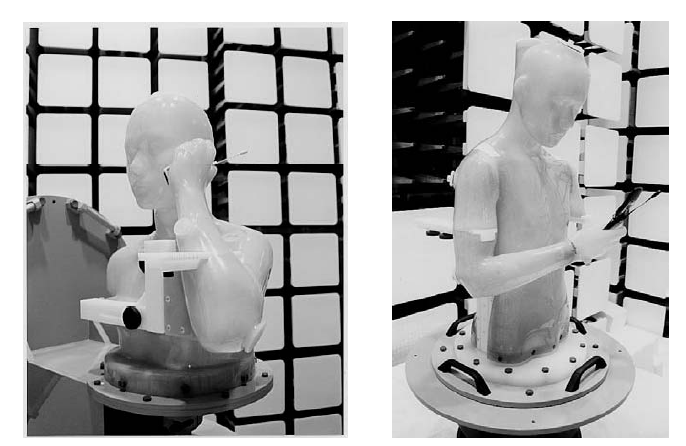
\includegraphics[scale=0.3]{./ContextoTecnologico/phantoms}}
    \subfigure[]{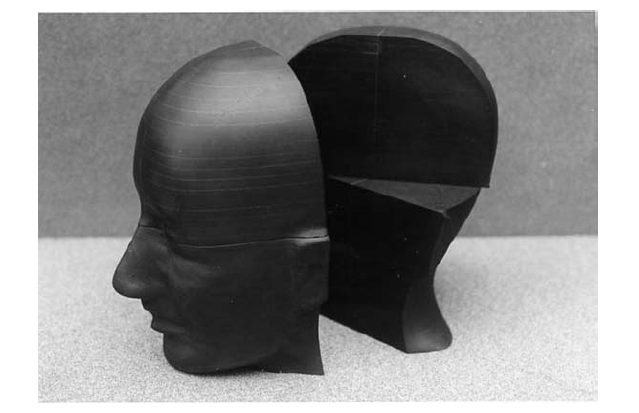
\includegraphics[scale=0.3]{./ContextoTecnologico/dry_phantom}}
    \caption{Distintos modelos de phantoms con apariencia humana \cite{yang}. En (a) modelos con posturas realistas humanas usando un teléfono móvil: a la izquierda en posición de conversación y a la derecha en posición de vista. En (b) un ejemplo de phantom seco.}
    \label{fig:fig3.2}
\end{figure}

\subsection{Modelos del cuerpo humano númericos para el estudio electromagnético}\label{subsec:modelos-del-cuerpo-humano-numericos-para-el-estudio-electromagnetico}

Para llegar a realizar un estudio exhaustivo de la medición registrada en un cuerpo, no sólo es necesario la creación de \textit{phantoms} o modelos físicos. Se necesitan estudios realizados por ordenador mediante medidas numéricas que contrasten los datos físicos obtenidos. En la actualidad, estos modelos numéricos son ampliamente utilizados a la par que los modelos físicos, ya que proporcionan un número importante de datos. Su principal fuente son los \textit{vóxels}. Un \textbf{\textit{vóxel}} es un píxel en tres dimensiones que representa la unidad mínima para la creación de modelos numéricos realizados por computador.

\begin{figure}[!htb]
    \centering
    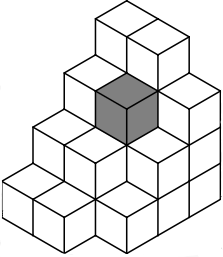
\includegraphics[scale=0.3]{./ContextoTecnologico/voxel}
    \caption{Ejemplo de vóxel cúbico. \cite{voxel}}
    \label{fig:fig3.3}
\end{figure}

Un vóxel forma parte de una matriz tridimensional necesaria para el procesamiento de imágenes. En nuestro caso, forman las imágenes que se usarán posteriormente para construir un modelo del cuerpo humano tridimensional. Los \textit{vóxels} pueden contener numerosos datos escalares que ayudan al posicionamiento, a calcular el volumen de la figura, etc.

En el campo de los DMI para personas, los \textit{voxel phantoms} ayudan a calcular las características de las antenas de los DMI cuando están cerca del cuerpo humano, formando un modelo real numérico, de gran exactitud y precisión.

\begin{figure}[!htb]
    \centering
    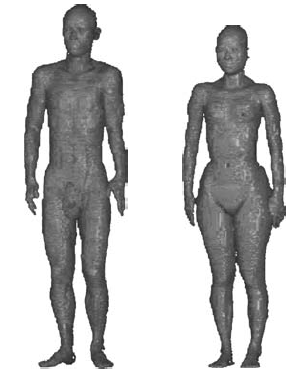
\includegraphics[scale=0.30]{./ContextoTecnologico/voxel_phantoms}
    \caption{Voxel phantoms de alta resolución de cuerpo entero. Modelos japoneses hombre y mujer. \cite{nagaoka}}
    \label{fig:fig3.4}
\end{figure}

\subsubsection{Técnicas para modelos numéricos para comunicaciones wireless}

Los modelos numéricos también se utilizan para el cálculo de índices SAR, pero también son utilizados como herramienta en análisis a frecuencia de microondas \cite{yang1}. Estos modelos permiten además aproximaciones semianalíticas, suponiendo que el cuerpo es un medio dieléctrico con pérdidas; esto da lugar a diversas técnicas de estudio:

\begin{itemize}
    \item  \textbf{Teoría geométrica uniforme de difracción} (\textit{Uniform Geometrical Theory of Diffraction, UTD}). Se basa en óptica geométrica y en teoría de difracción.
    \item  \textbf{Técnica de trazo de rayos o RT}. Puede ser usada para determinar la fuerza de la señal recibida y perfiles de potencia en situaciones donde la longitud de onda es pequeña en relación con el tamaño del entorno de propagación.
    \item \textbf{Método de los momentos o MoM}. Es una técnica para resolver ecuaciones con integrales complejas reduciéndolas a un sistema de ecuaciones lineales más simple. Puede ser usada en el dominio tanto de la frecuencia como del tiempo para analizar de manera bastante exacta estructuras estrechas.
    \item \textbf{Método de los elementos finitos o FEM}. La idea básica de esta técnica es dividir las estructuras electromagnéticas en un número de elementos de forma variante, tales como rectangulares o triangulares. Cada elemento tiene un valor de campo asociado, los cuales conforman una matriz de pesos donde calcular autovalores.
    \item \textbf{Método de las diferencias finitas en el dominio del tiempo o FDTD Method}. Método que destacaremos a continuación ya que es implementado por el software que vamos a utilizar para nuestro estudio.
\end{itemize}

\subsubsection{Método de las diferencias finitas en el dominio del tiempo. FDTD Method}

Este método es uno de los más conocidos dentro de los métodos numéricos para problemas de condiciones de contorno difíciles de resolver. Ha sido aplicado además a problemas electromagnéticos durante muchos años~\cite{yang}. Al igual que FEM, parte de la divisón de estructuras electromagnéticas en un conjunto de pequeñas celdas para poder así obtener de manera idónea los cálculos de condiciones de contorno complicados en medios no homogéneos.

Una de las razones por las cuales el método FDTD ha visto un rápido crecimiento en su uso, ha sido su complejidad en pasos de computación\footnote{Número de instrucciones necesarias de un programa para realizar un cálculo computacional.}, siendo esta O(n). Otros métodos, como el MoM o FEM, necesitan O(n$^{2}$) de complejidad, es decir, necesitan n veces más cálculos computacionales que en FDTD. Los resultados con un rango de frecuencias amplio, se pueden conseguir fácilmente a través de la implementación de la Transformada Rápida de Fourier (FFT) en el dominio temporal, lo que abarata el cálculo de los datos a obtener~\cite{yang}.

Sin embargo, el FDTD tiene sus inconvenientes. Requiere que todo el dominio de trabajo sea dividido en una malla compuesta por celdas, las cuales deben ser más pequeñas que la longitud de onda más corta y más pequeñas que la medida más diminuta del modelo. Además, como muchos de los elementos estructurales electromagnéticos son curvos, los límites o perfiles de las celdas no serán suaves, sino rugosas, con cortes. En este aspecto, el método FDTD no es tan flexible como el FEM.


\section{Bandas de frecuencia para los sistemas de comunicación de los dispositivos médicos implantables}\label{bandas}

En los capítulos~\ref{ch:intro} y~\ref{ch:contexto} se ha mencionado que la tecnología utilizada en los orígenes de los DMI para que los dispositivos se comunicaran, era el enlace inductivo. Debido a sus limitaciones en capacidad y distancia de transmisión de datos, se han establecido dos bandas certificadas de radiofrecuencia para DMI que minimizan esas dos limitaciones. Nos referimos a la banda \textbf{MICS} (\textit{Medical Implant Communication Service}) y la banda \textbf{ISM} (\textit{Industrial, Scientific and Medical band}).

\subsection{Banda MICS}

Tanto el Instituto Europeo de Estandarizaciones en Telecomunicación, conocido como ETSI (\textit{European Telecommunications Standards Institute}), como el FCC (\textit{Federal Communications Commission}) por parte de Estados Unidos, recogen la estandarización de la banda MICS~\cite{mics}. Nos centraremos principalmente en el estándar definido en ETSI, el cual establece dos principales usos para esta banda:

\begin{itemize}
    \item La comunicación entre un dispositivo implantable y un dispositivo que funciona como estación base que recoge la información que vierte el primero.
    \item La comunicación entre varios (dos o más) dispositivos que se encuentran implantados en un mismo cuerpo.
\end{itemize}

Sin embargo, el estándar no recoge otro uso también destacable y que es posible realizar: la comunicación entre dispositivos implantables que se sitúan en diferentes cuerpos~\cite{yang9}.

La frecuencia de trabajo de esta banda se encuentra entre los \textbf{402 MHz} y los \textbf{405 MHz}. Este espectro de 3 MHz se reparte en 10 canales, con lo que el máximo ancho de banda disponible es de 300 KHz en una única transmisión. Esto es una desventaja importante para esta banda ya que si se trabaja en comunicaciones \textit{full-duplex}, es decir todo dispositivo puede transmitir y recibir información a la vez, el ancho de banda necesario para cada dispositivo es pequeño, lo que reduce la tasa de información considerablemente. Debido a esto, tenemos otra posibilidad para utilizar todo el ancho de banda: utilizar \textit{half-duplex}, es decir que en cada momento el dispositivo sólo puede transmitir o recibir información (no a la vez), y que cada dispositivo utilice totalmente el ancho de banda en su turno de transmisión. Esta última posibilidad limita tanto la recogida de información como la comunicación entre dispositivos.

Como los 300 KHz de ancho de banda total en esta banda supone una restricción importante, se ha establecido que en los límites de emisión, la potencia debe ser 20 dB menor que el máximo nivel. La potencia radiada equivalente\footnote{El nivel máximo de campo emitido en cualquier dirección debería ser igual o menor a la de un dipolo resonante a la misma distancia con máxima directividad siendo alimentado por una señal de 25$\mu$W.} (ERP) es de 25$\mu$W. Según el estándar MICS para ETSI~\cite{mics} los niveles de ERP deben medirse a través de simulaciones recogidas en implantes colocados sobre un objeto con forma de torso humano. No existen estandarizaciones para implantes usados principalmente en otras partes del cuerpo, como son brazos, piernas o en la cabeza. De acuerdo con el estándar, cada implante diseñado y fabricado en esta banda, sin importar dónde irá colocado, debe ser probado con la misma simulación de torso humano anteriormente descrita.

Existe otro inconveniente para esta banda de frecuencias. El Servicio de Apoyo Meteorológico o METAIDS (\textit{Meteorological Aids Service}), utiliza esta banda para transmitir información de la previsión meteorológica desde antenas colocadas en globos aerostáticos hasta antenas que recogen la información en la superficie de la Tierra. Por esta razón, la banda MICS está especificada únicamente para su uso en interiores y no para su uso en exteriores~\cite{yang9,mics}. Posteriormente, la ITU-T ha propuesto una recomendación de cómo debe repartirse y usarse el espectro en la banda de 401 MHz a 406 MHz~\cite{itut}, en el cual la banda MICS queda dispuesta entre los 402 MHz y los 405 MHz: el resto es para el servicio METAIDS.

\subsection{Banda ISM}\label{subsec:banda-ism}

La banda ISM es usada también para la comunicación entre implantes o DMI. Trabaja en las mismas frecuencias que algunos estándares de IEEE~\cite{IEEE} como el 802.11 (Wi-Fi)~\cite{wifi}, 802.15 (Bluetooth)~\cite{bluetooth} por poner unos ejemplos.

De acuerdo de nuevo a ETSI~\cite{etsi}, el máximo ERP en la banda ISM es de 100 mW. Las tecnologías de reparto de frecuencias que son posibles de utilizar en esta banda son espectro ensanchado, espectro ensanchado por salto de frecuencias o FHSS y espectro ensanchado por secuencia directa o DSSS. La banda de frecuencias se encuentra entre los 2.4 y los 2.4835 GHz.

La desventaja fundamental de esta banda de trabajo es el solapamiento que existe con otros estándares y tecnologías: esto hace que sea una banda con riesgos en seguridad e interoperabilidad. Con respecto a la banda MICS, que trabaja en torno a los 400 MHz como hemos mencionado antes, la atenuación de las ondas de propagación que presentan en la banda ISM ante un cuerpo humano es mucho mayor. De esta manera, esta banda es posible utilizarla para el uso de dispositivos implantados alrededor del cuerpo y no en su interior, ya que se aprovecha de las ondas que se propagan por la superficie del cuerpo~\cite{conway,yang9}. El caso más general, es utilizar esta banda para sincronizar y activar al DMI cuando se vaya a interactuar con él; es entonces cuando se utiliza la banda MICS para intercambiar información. Un ejemplo claro lo podemos ver en la siguiente sección.

Sin embargo, el problema al que hacíamos mención en la banda MICS, el poco ancho de banda disponible, aquí es solventado, ya que tenemos un ancho de banda muy superior. Dos o más dispositivos pueden transmitir a la vez, pueden establecerse comunicaciones \textit{full-duplex} sin problemas junto a la utilización además de cualquier tecnología de las arriba citadas, FHSS, DSSS, etc., con lo que tenemos la posibilidad de aumentar los recursos de estos dispositivos.

\subsection{Comparación entre las bandas MICS e ISM}\label{subsec:comparacion}

En la \textit{tabla \ref{tab:tabla3.2}} se presenta una tabla comparativa de ambos estándares, donde se recogen las bandas de frecuencia, usos, potencia, tipo de comunicación, etc.

\begin{table}[h]
    \centering\scalebox{0.8}{
        \begin{tabular}{| c | c | c | c | c | c |}
            \hline
            \large{\textbf{Estándar}}           & \textbf{MICS}               & \textbf{ISM}                     \\
            \hline
            \hline
            \large{\textbf{Frecuencias}}        & 402 - 405 MHz               & 2.4 - 2.4835 GHz                 \\
            \large{\textbf{de trabajo}}         &                             &                                  \\
            \hline
            \large{\textbf{Potencia}}           & 25 $\mu$W                   & 100 mW                           \\
            \large{\textbf{máxima}}             &                             &                                  \\
            \hline
            \large{\textbf{Recogido}}           & ITU-T                       & ITU-T                            \\
            \large{\textbf{en}}                 & ETSI                        & ETSI                             \\
            & FCC                         & FCC                              \\
            %\hline
            %\large{\textbf{Uso}} & Tejidos interior del cuerpo & Tejidos superficiales del cuerpo \\
            %\large{\textbf{científico/médico}} & & \\
            \hline
            \large{\textbf{Velocidad}}          & Kbps                        & Mbps                             \\
            \large{\textbf{de bits}}            &                             &                                  \\
            \hline
            \large{\textbf{Ancho}}              & 300 KHz                     & MHz                              \\
            \large{\textbf{de banda}}           &                             &                                  \\
            \hline
            \large{\textbf{Tipo}}               & \textit{half-duplex}        & \textit{full-duplex}             \\
            \large{\textbf{de transmisión}}     &                             &                                  \\
            \hline
            \large{\textbf{Reparto}}            & N/A                         & FHSS, DSSS                       \\
            \large{\textbf{de frecuencias}}     &                             &                                  \\
            \hline
            \hline
        \end{tabular}}
    \caption{Características comparativas de las bandas MICS e ISM vistas anteriormente.}
    \label{tab:tabla3.2}
\end{table}

Como ejemplo práctico a las dos bandas vistas, podemos ver un modelo de chip de la empresa \textbf{\textit{Microsemi}}, antigua \textit{Zarlink Semiconductor}. En la ilustración de la \textit{fig. \ref{fig:fig3.5}} se puede ver. Este modelo utiliza la banda ISM para \textit{despertar} al dispositivo implantable que está junto al chip: el dispositivo entra en modo \textit{idle} o inactivo cuando después de un cierto tiempo no recibe ninguna orden de algún dispositivo externo. Una vez despertado, el dispositivo recoge toda la información necesaria por el uso de la banda MICS y utiliza esta misma banda para enviar dicha información al dispositivo externo que le ha despertado. En definitiva:

\begin{itemize}
    \item El equipo externo de monitorización manda una señal en la banda ISM al dispositivo del chip para que se active y empiece a funcionar.
    \item El dispositivo del chip, recoge la información a través de la banda MICS y la entrega al equipo externo por la misma vía.
\end{itemize}

\begin{figure}[!htb]
    \centering
    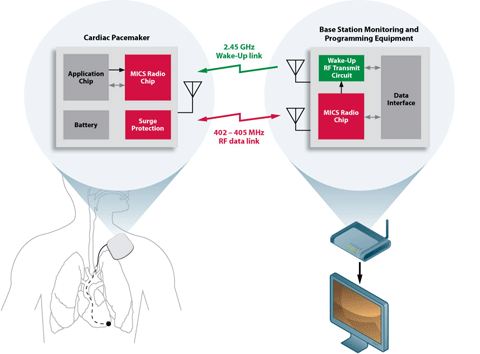
\includegraphics[scale=0.6]{./Introduccion/medical-cardicpacemaker}
    \caption{Ilustración ejemplo de la estructura de comunicación de un chip de la empresa \textit{Microsemi} \cite{zarlink}.}
    \label{fig:fig3.5}
        % http://www.zarlink.com/zarlink/hs/22122.htm
\end{figure}
